\chapter{Learning useful representation of data}\label{ch:learningrepresentations}



In this chapter, we introduce the basic ideas from the representation learning.
We identify properties of \textit{good data representations} and illustrate three common representation learning approaches.




\section{Introduction}


As we have seen in Section \ref{sec:intro_ml} of Chapter \ref{ch:introduction}, machine learning intuitively corresponds to \textit{discovering} of function \textit{f} mapping the input data $X$ to some target concept $y$:

\begin{equation}
	f(X) = y.
	\label{eq:ml}
\end{equation}


This also illustrates why we care so much about the representation of data: if the information in $X$ is insufficient in capturing the information relevant to the mapping itself, whatever \textit{f} we learn  is doomed to be a bad one.
As one relies on \gls{ml} in scenarios when one has little or no knowledge of \textit{f}, it is very difficult, if not impossible, to know in advance which information is relevant for the mapping.
Deploying \gls{ml} solution in practice, thus, requires a lot of manual work just to identify the relevant information for the task.



A pleasing property of introducing a representation learning component in a \gls{ml} pipeline is that is \textit{surpasses the limitation of fixed data representation}.
It thus generalises the machine learning equation (Equation \ref{eq:ml}) to:

\begin{equation}
	f(m(X)) = y
\end{equation}

where, in addition to the decision function \textit{f}, we include the representation mapping function \textit{m}.
Moreover, several mapping function can be \textit{stacked} together to perform multiple representation learning steps.







\section{Representation learning principles}


The core focus of representation learning is on \textit{learning} the function(s) \textit{m}$_{(i)}$.
By the time of writing of this thesis, several thousands of different representation learning methods exist in the literature \cite{Goodfellow2016}.
In this section we illustrate the principles of representation learning on a few prototypical approaches.


\subsection{Artificial neural networks}



\newglossaryentry{ann}{name={ANN},description={Artificial Neural Networks}}
Representation learning as a field has risen from the advances in \textit{artificial neural networks} (\gls{ann}).
Til this day, almost all representation learning methods are developed within the framework of \gls{ann}s.


\gls{ann} (Figure \ref{fig:ann}) is a simple mathematical formalisation of \textit{human brain}.
It consists of a \textit{network} of mutually connected \textit{artificial neurons}, also known as \textit{perceptrons} (circles in Figure \ref{fig:ann}).
The interactions between neurons are dictated by their connections (edges connecting circles in Figure \ref{fig:ann}).


An \gls{ann} in Figure \ref{fig:ann} consists of three \textit{layers}: an \textit{input layer} which takes the data $X$, an \textit{output layer} capturing the target concept $y$ and a \textit{hidden layer} performing the representation transformation.
\gls{ann} operates by activating neurons in different amounts depending on the input data -- similar to the human brain.
Each neuron in the hidden layer is connected to all of the input neurons, but with different \textit{strengths} of connections.
In formal terms, the amount of activation of any individual neuron equals

\begin{equation}
	a(X) = n(\sum_{i=1}^N w_i \times x_i)
\end{equation} 

where $w_i$ stands for the strength of the connection, and $x_i$ is the value of an input neuron.
The function \textit{n} is any non-linear function determining the activation based on the weighted sum of the activations of the input neurons, i.e., the data.




\begin{figure}
	\centering
	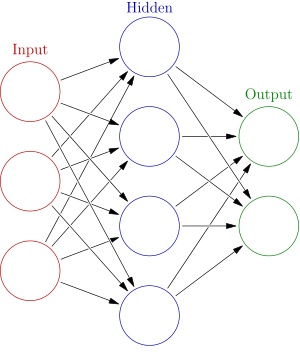
\includegraphics[width=.5\linewidth]{ann}
	\caption{Artificial neural network}
	\label{fig:ann}
\end{figure}


The task of learning \gls{ann}s the one of learning the strengths of connections given fixed structure of an \gls{ann}s.
Once learned, the activations of the neurons in the hidden layer represents the new representation of data.


\gls{ann}s belong to the \textbf{supervised} branch of representation learning methods, i.e., they learning new representation tailored specifically for the given task ($y$).




\subsection{Auto-encoders}


A very different approach to learning representations are \textit{auto-encoders} \cite{Hinton504}.
Auto-encoders belong to the \textbf{unsupervised} branch of representation learning methods which do not consider a particular supervised, target, information when learning representations.
A benefit of unsupervised representation learning is that the new representations can be used for many tasks as they are not tailored for a certain task.


Learning new representations in an unsupervised way is substantially more difficult than the supervised case.
Given the labelled information, one can verify how useful every feature in the new representation is  by, for instance, evaluation to which extent each feature contributes towards distinguishing different target labels.
In the unsupervised case, we have no access to such information.
The question then is: \textit{What constitutes a good representation if we don't know the target task?}


\begin{figure}
	\centering
	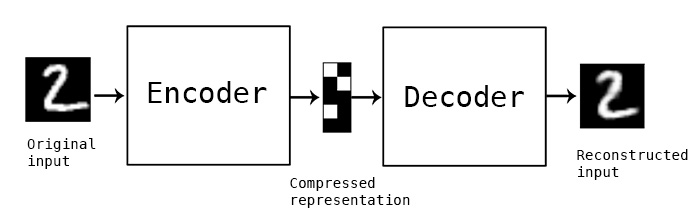
\includegraphics[width=.8\linewidth]{ae}
	\caption{Auto-encoder}
	\label{fig:ae}
\end{figure}



Auto-encoders introduce a practical way to circumvent tackling that difficult question first.
Auto-encoders are \gls{ann}s that learn data representation by trying to compress the original data such that the original data can be reliably reconstructed from the compressed representation.
Two parts of an auto-encoder (Figure \ref{fig:ae}) are \textit{encoder}, mapping the original data to a new representation, and a \textit{decoder} mapping the latent representation of data back to the original representation.
It is important to note that training auto-encoders does not require any change in learning \gls{ann}s, except of requirement that the \gls{ann} reconstructs its own input $y \approx X$.




The key in successfully learning representation with auto-encoders lies in imposing certain constraints on the hidden layer of the auto-encoder.
Otherwise, without the constraints, nothing prevents the auto-encoders to learn the \textit{identity mapping} which would guarantee the perfect reconstruction.
The most common way of preventing the learning of identity mapping is to force the auto-encoders to be \textit{compressive}; this is achieved by restricting the dimension of the hidden layer to be \textit{smaller} than the dimension of the input data.
This way, the auto-encoder is forced to exploit the patterns in data in order to maximise the reconstruction from the latent representation.






\subsection{Properties of good data representation}


The success of representation learning initiated a lot of work towards understanding the properties that constitute a good data representation \cite{Bengio2013RLR}.
Here we provide a concise overview of the most important properties.


\textbf{multiple explanatory factors}

\textbf{a hierarchical organisation of explanatory factors}

\textbf{shared factors across tasks}

\textbf{manifolds}

\textbf{natural clustering}

\textbf{simplicity of factor dependencies}

\textbf{sparsity}








\section{Learning representations of relational data}


The few examples discussed in the previous section consider learning representation from tabular data only.
In this section we provide a brief overview of the main ideas present in transferring these ideas towards relational data.


\subsection{Knowledge graph embeddings}

\newglossaryentry{kge}{name={KGE},description={Knowledge Graph Embeddings}}

By far the largest group of methods for representation learning with relational data are \textit{knowledge graph embeddings}.
The core idea behind \gls{kge}s is to replace the symbolic data representation common in multi-relational and graph data with a numerical approximation, i.e., they associate an $n-$dimensional vector (or a matrix) with each symbol in the data.


 \begin{figure}
	\centering
	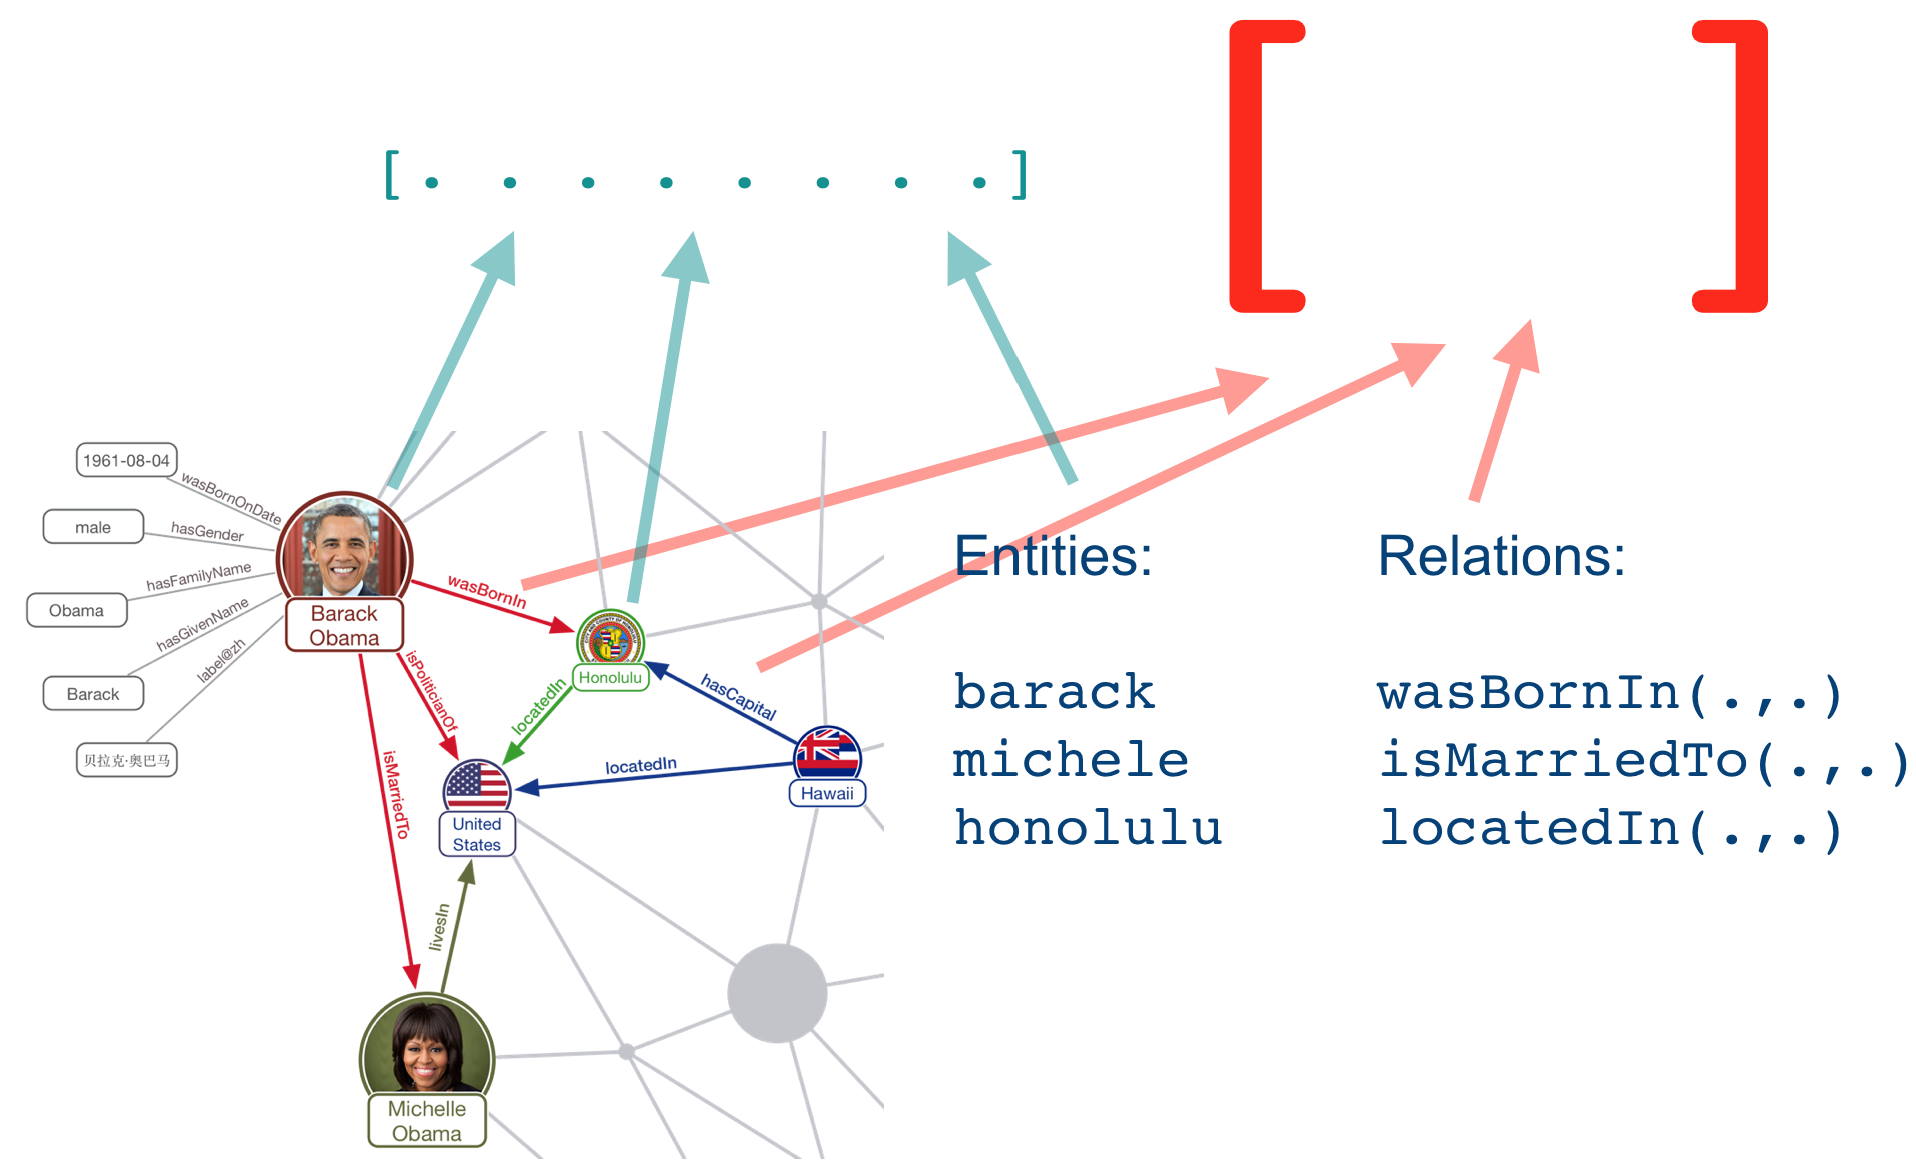
\includegraphics[width=.8\linewidth]{illustrationembeddings}
	\caption{Illustration of the embedding approaches}
	\label{fig:emb}
\end{figure}


The representation learning task of \gls{kge}s is the one of learning the numerical representation of symbols (Figure \ref{fig:emb}).
In order to find a good numerical representation, \gls{kge} associate a \textit{score} with 
 
 





\subsection{Capturing data properties with random walks}



\subsection{Logical approaches}



%%%%%%%%%%%%%%%%%%%%%%%%%%%%%%%%%%%%%%%%%%%%%%%%%%
% Keep the following \cleardoublepage at the end of this file, 
% otherwise \includeonly includes empty pages.
\cleardoublepage

% vim: tw=70 nocindent expandtab foldmethod=marker foldmarker={{{}{,}{}}}
